% -*-coding: utf-8 -*-
% Держать в начале каждого файла!

\documentclass[a4paper, 12pt]{extarticle}
\usepackage{metod}

\MTDSetPhysSection{Механика}
\MTDSetTitle{Изучение законов поступательного движения твердого тела}
\MTDDesignator{М--2}
\MTDSetGrade{10}

\MTDSetAuthors{И.~Н.~Грачева, В.~И.~Гребенкин, А.~Е.~Иванов, И.~А.~Коротова,
Е.~И.~Красавина, А.~В.~Кравцов, Н.~С.~Кулеба, Б.~В.~Падалкин,
Г.~Ю.~Шевцова, Т.~С.~Цвецинская}

\MTDSetEditorsGenCase{И.~Н.~Грачевой, А.~Е.~Иванова, А.~В.~Кравцова}

\begin{document}

\MTDTitlePage
\MTDInfoPage

\setcounter{section}{2}

\subsection{Цель работы}
Целью работы является экспериментальная проверка законов поступательного равноускоренного движения твердого тела.

\subsection{Основные теоретические сведения}
Твердым телом в механике называется такое тело, у которого во время движения не изменяются расстояния между частицами, составляющими тело.

Движение твердого тела называется поступательным, если прямая, проведенная через две любые точки тела, остается при движении параллельной самой себе.

При поступательном движении все частицы тела имеют одинаковые по величине и направлению скорости и ускорения. Поэтому движение тела можно рассматривать как движение одной материальной точки, имеющей массу всего тела. В качестве такой материальной точки обычно выбирают центр масс тела.

В случае равноускоренного поступательного движения твердого тела (материальной точки) уравнение движения и уравнение для скорости имеют вид:

\begin{align}
\label{eq:m2-uni-acc-motion}
\begin{split}
\vec{r} &= \vec{r_0} + \vec{v_0}t + \frac{\vec{a}t^2}{2} \\ %запятая?
\vec{v} &= \vec{v_0} + \vec{a}t,
\end{split}
\end{align}
где $\vec{r}$ "--- радиус-вектор конечного положения тела; \\
$\vec{r_0}$ "--- радиус-вектор начального положения тела; \\
$\vec{v_0}$ "--- начальная скорость тела; \\
$\vec{v}$ "--- скорость тела в момент времени $t$; \\
$\vec{a}$ "--- ускорение. %<s>теперь непонятно, надо запятую или точку с запятой</s> отступы нормальные или чего

Для прямолинейного равноускоренного движения с нулевой начальной скоростью пройденный путь и скорость зависят от времени движения как

\begin{align}
\label{eq:m2-uni-acc-lin-motion}
\begin{split}
s &= \frac{at^2}{2} \\ %запятая?
v &= at.
\end{split}
\end{align}

\subsection{Описание экспериментальной установки}
\begin{figure}[h] %как сделать сбоку
\begin{center}
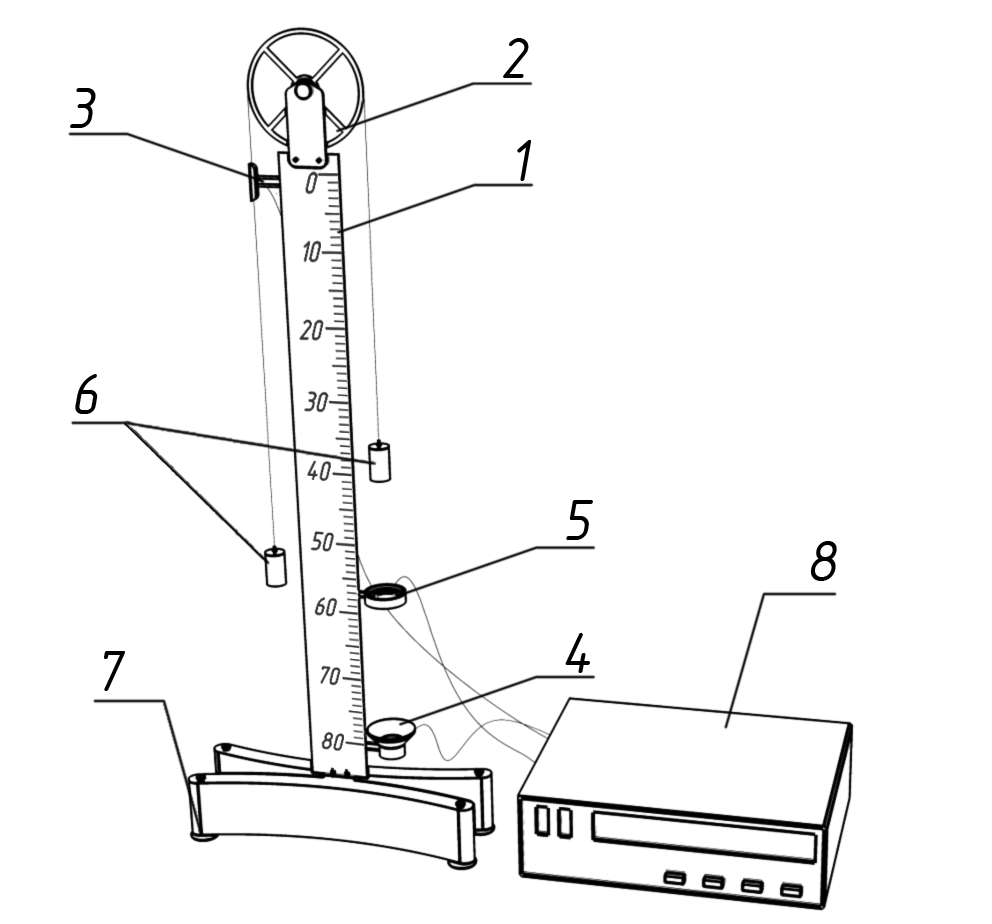
\includegraphics[keepaspectratio=true]{M2-AtwoodsMachine}
\end{center}
\caption{Схема экспериментальной установки \label{fig:m2-atwood-machine}}
\end{figure}
Работа выполняется на машине Атвуда (рис.~\ref{fig:m2-atwood-machine}).

Установка состоит из вертикальной стойки~\emph{1} с сантиметровыми делениями и блока~\emph{2}, укрепленного в подшипнике. Через блок переброшена нить с грузами~\emph{6} одинаковой массы. Нить зажимается электромагнитом~\emph{3}, электропитание которого включается и выключается с пульта электронного секундомера~\emph{8}. Один из грузов~\emph{6} может проходить через кольцо~\emph{5}, на котором установлен контакт <<Старт>> секундомера. На приемной площадке~\emph{4} установлены контакты <<Стоп>> секундомера.
% ИЗМ: секундомер стал восьмым

\subsection{Методика выполнения работы}
Правый груз~\emph{6} с дополнительным грузом устанавливается на некоторой высоте $s$ над приемной площадкой. При размыкании электромагнита начинается равноускоренное движение этого груза вниз, и происходит пуск электронного секундомера. При касании груза приемной площадки~\emph{4} происходит остановка секундомера. Таким образом происходит измерение времени прохождения грузом пути $s$. Пользуясь уравнениями~\eqref{eq:m2-uni-acc-lin-motion} для случая $v_0 = 0$, можно рассчитать конечную скорость $v_k$ груза в момент удара о приемную площадку~\emph{4}:
\begin{equation}
\label{eq:m2-final-speed}
v_k = \frac{2s}{t}.
\end{equation}

Затем правый груз~\emph{6} с дополнительным грузом устанавливают на том же расстоянии~$s$ над кольцом~\emph{5}. Кольцо~\emph{5} задерживает дополнительный груз, который, касаясь кольца, замыкает цепь пуска секундомера. После снятия дополнительного груза грузы продолжают двигаться равномерно со скоростью, равной~$v_k$. При ударе груза о приемную площадку, расположенную на расстоянии~$s'$ от кольца, секундомер останавливается. Скорость равномерного движения~$v'$ определяется выражением
\begin{equation}
\label{eq:m2-constant-motion-speed}
v' = \frac{s'}{t'},
\end{equation}
где $t'$ "--- время прохождения грузом расстояния между кольцом~\emph{5} и приемной площадкой~\emph{4}. %ИЗМ: наиболее вероятная формула

Если предположение о постоянстве ускорения при движении груза с дополнительным грузом справедливо, то $v_k = v'$. Правильная работа машины Атвуда зависит от точности уравновешивания грузов~\emph{6} и тщательности выставления стойки~\emph{1} в вертикальное положение уравнительными винтами~\emph{7}. Груз должен проходить через кольцо~\emph{5}, не задевая его, и ударяться о центр приемной площадки~\emph{4}, а дополнительный груз "--- легко сниматься кольцом. %ИЗМ: "ударяться о приемную площадку 4 в центре ее" -> "ударяться о центр приемной площадки 4"

\subsection{Порядок выполнения работы}
\begin{enumerate}
\item Во время домашней подготовки к работе начертите в лабораторном журнале таблицу~\ref{tab:m2-res-exp}.

\begin{table}[h] %вот так наверное ничего в плане ширины
\caption{\label{tab:m2-res-exp}}
\begin{flushright}
\begin{tabular}{|c|>{\centering\arraybackslash} m{0.25cm}|>{\centering\arraybackslash} m{0.25cm}|>{\centering\arraybackslash} m{0.25cm}|c|c|c|c|>{\centering\arraybackslash} m{0.25cm}|>{\centering\arraybackslash} m{0.25cm}|>{\centering\arraybackslash} m{0.25cm}|c|c|c|}
\hline
\multirow{2}*{$s$,~\Units{м}} & \multicolumn{3}{c|}{$t$,~\Units{c}} & \multirow{2}*{\hspace{3pt}$\MTDMean{t},$~\Units{c}} & \multirow{2}*{$v_k$,~\Units{м/c}} & \multirow{2}*{$\Delta v_k$,~\Units{м/c}} & \multirow{2}*{$s'$,~\Units{\text{м}}} & \multicolumn{3}{c|}{$t'$,~\Units{c}} & \multirow{2}*{\hspace{3pt}$\MTDMean{t'},$~\Units{c}} & \multirow{2}*{$v'$,~\Units{м/c}} & \multirow{2}*{$\Delta v'$,~\Units{м/c}} \\ \cline{2-4} \cline{9-11}
   & 1 & 2 & 3 & & & & & 1 & 2 & 3 & & &\\ \hline
0,6 & & & & & & & & & & & & &\\ \hline
0,4 & & & & & & & & & & & & &\\ \hline
0,2 & & & & & & & & & & & & &\\ \hline
\end{tabular}
\end{flushright}
\end{table}

\item Ознакомьтесь с установкой и запишите технические характеристики электронного секундомера.
\item Убрав кольцо~\emph{5}, отрегулируйте положение машины Атвуда, чтобы правый груз опускался на середину приемной площадки~\emph{4}.
\item Надев на правый груз дополнительный груз, по три раза измерьте время движения груза с высот $s_1 = 0,6~\text{\Units{м}}$, $s_2 = 0,4~\text{\Units{м}}$ и $s_3 = 0,2~\text{\Units{м}}$. Результаты измерений запишите в таблицу~\ref{tab:m2-res-exp}.
\item Рассчитайте конечные скорости движения груза для трех значений пути по формуле~\eqref{eq:m2-final-speed}. Определите погрешности значений конечных скоростей по выражению
\begin{equation}
\label{eq:m2-final-speed-error}
\Delta v_k = \MTDMean{v_k}\sqrt{E_s^2 + E_t^2},
\end{equation}
где $E_s = \Delta s / s$; $E_t = \Delta t / t$; \\ %мб \dfrac
$\Delta s$ "---  приборная погрешность, равная половине цены деления стойки; \\ %ррр, не знаю, что делать с этими пояснениями к формулам, как их форматировать
$\Delta t$ "--- погрешность измерения времени, рассчитываемая по методике, изложенной в разделе~В.4 настоящего сборника. %раздел В.4
\item Постройте график зависимости $v(t)$. По наклону этого графика определите ускорение~$a$, учитывая, что
\begin{equation}
\label{eq:m2-acceleration}
a = \frac{dv}{dt},
\end{equation}
т.~е. необходимо определить тангенс угла наклона графика~$v(t)$ к оси~$t$. Пользуясь формулами раздела~В.5 настоящего сборника, определите погрешность измерения ускорения $\Delta a$. %раздел В.5
\item Поставьте кольцо~\emph{5} на таком расстоянии от приемной площадки~\emph{4}, чтобы при самом высоком положении груза~\emph{6} последний находился на расстоянии~$s_1 = 0,6~\text{\Units{м}}$ от кольца~\emph{5}. Измерьте расстояние~$s'$, результат запишите в таблицу~\ref{tab:m2-res-exp}.
\item Измерьте по три раза время прохождения грузом~\emph{6} расстояния~$s'$ при $s_1 = 0,6~\text{\Units{м}}$, $s_2 = 0,4~\text{\Units{м}}$, $s_3 = 0,2~\text{\Units{м}}$. Результаты запишите в таблицу~\ref{tab:m2-res-exp}.
\item По формуле~\eqref{eq:m2-constant-motion-speed} рассчитайте скорость $v'$ для всех $s$. Определите погрешность измерения $v'$ по выражениям, аналогичным приведенным в п.~5.
\item Постройте график зависимости $v'(t)$ \textbf{(не от $\boldsymbol{t'}$)}, где $t$ "--- время движения груза с высоты $s$, взятое из предыдущего эксперимента. По наклону этого графика определите ускорение $a$. Пользуясь формулами раздела~В.5 настоящего сборника, определите погрешность измерения ускорения $\Delta a$.
\item Сравните полученные в пп.~6~и~10 результаты и сделайте вывод о характере движения груза. %раздел В.5
\item По данным работы постройте график зависимости $s(t)$.
\item Напишите заключение к работе.
\end{enumerate}

\subsection{Контрольные вопросы}
\begin{enumerate}
\item Как относятся между собой пути, проходимые грузом при равнопеременном движении за последовательные равные промежутки времени?
\item Как связаны конечная скорость (формула~\eqref{eq:m2-final-speed}) со средней скоростью при равнопеременном движении?
\item Найдите с помощью графика $s(t)$ чему равна мгновенная скорость груза в точке $(t_3, s_3)$. %ИЗМ: (s_3, t_3) -> (t_3, s_3) | "покажите" -> "найдите"
\end{enumerate}

\end{document}
